
\documentclass[letterpaper,english,10pt]{article}

\usepackage{%
	amsfonts,%
	amsmath,%	
	amssymb,%
	amsthm,%
	babel,%
	bbm,%
	%biblatex,%
	caption,%
	centernot,%
	color,%
	enumerate,%
	%enumitem,%
	epsfig,%
	epstopdf,%
	etex,%
	fancybox,%
	framed,%
	fullpage,%
	%geometry,%
	graphicx,%
	hyperref,%
	latexsym,%
	mathptmx,%
	mathtools,%
	multicol,%
	pgf,%
	pgfplots,%
	pgfplotstable,%
	pgfpages,%
	proof,%
	psfrag,%
	%subfigure,%	
	tikz,%
	times,%
	ulem,%
	url,%
	xcolor,%
	mathpazo
}

\definecolor{shadecolor}{gray}{.95}%{rgb}{1,0,0}
\usepackage[margin=1in,top=0.75in]{geometry}
\usepackage[mathscr]{eucal}
\usepgflibrary{shapes}
\usepgfplotslibrary{fillbetween}
\usetikzlibrary{%
  arrows,%
  backgrounds,%
  chains,%
  decorations.pathmorphing,% /pgf/decoration/random steps | erste Graphik
  decorations.text,% 
  matrix,%
  positioning,% wg. " of "
  fit,%
  patterns,%
  petri,%
  plotmarks,%
  scopes,%
  shadows,%
  shapes.misc,% wg. rounded rectangle
  shapes.arrows,%
  shapes.callouts,%
  shapes%
}

%\pgfplotsset{compat=newest} %<------ Here
\pgfplotsset{compat=1.11} %<------ Or use this one

\theoremstyle{plain}
\newtheorem{thm}{Theorem}[section]
\newtheorem{lem}[thm]{Lemma}
\newtheorem{prop}[thm]{Proposition}
\newtheorem{cor}[thm]{Corollary}
\newtheorem{clm}[thm]{Claim}

\theoremstyle{definition}
\newtheorem{axiom}[thm]{Axiom}
\newtheorem{defn}[thm]{Definition}
\newtheorem{conj}[thm]{Conjecture}
\newtheorem{exmp}[thm]{Example}
\newtheorem{exerc}[thm]{Exercise}
\newtheorem{assum}[thm]{Assumptions}

\theoremstyle{remark}
\newtheorem{rem}[thm]{Remark}
\newtheorem{note}[thm]{Note}

\newcommand{\Cov}{\operatorname{Cov}}
%\newcommand{\det}{\operatorname{det}}
\newcommand{\Real}{\mathbb{R}}
\newcommand{\tr}{\operatorname{tr}}
%\newcommand{\Var}{\operatorname{Var}}

\DeclareMathOperator{\sign}{sign}
%\renewcommand{\proof}[1]{\begin{proof}#1\end{proof}}
\newcommand{\EQ}[1]{\begin{equation*}#1\end{equation*}}
\newcommand{\EQN}[1]{\begin{equation}#1\end{equation}}
\newcommand{\eq}[1]{\begin{align*}#1\end{align*}}
\newcommand{\meq}[2]{\begin{xalignat*}{#1}#2\end{xalignat*}}
\newcommand{\norm}[1]{\left\lVert#1\right\rVert}
\newcommand{\abs}[1]{\left\lvert#1\right\rvert}
\newcommand{\expect}[1]{\mathbb{E}\left[{#1}\right]}
\newcommand{\prob}[1]{\mathbb{P}\left[{#1}\right]}
\newcommand{\given}{\; \big\vert \;} 
\newcommand{\set}[1]{\left\{#1\right\}} 
\newcommand{\indicator}[1]{\mathbb{1}_{\set{#1}}} 
\newcommand{\inner}[1]{\left\langle#1\right\rangle}
\newcommand{\red}[1]{\textcolor{red}{#1}} 
\newcommand{\E}[1]{\mathbb{E}\left[#1\right]}
\newcommand{\Var}[1]{\operatorname{Var}\left[#1\right]}

\newcommand{\D}{\mathbb{D}}
%\newcommand{\E}{\mathbb{E}}
\newcommand{\N}{\mathbb{N}}
\renewcommand{\P}{\mathbb{P}}
\newcommand{\Q}{\mathbb{Q}}
\newcommand{\R}{\mathbb{R}}
\newcommand{\Z}{\mathbb{Z}}

\newcommand{\bU}{\mathbf{1}}
\newcommand{\bx}{\mathbf{x}}

\newcommand{\cB}{\mathcal{B}}
\newcommand{\cC}{\mathcal{C}}
\newcommand{\cD}{\mathcal{D}}
\newcommand{\cF}{\mathcal{F}}
\newcommand{\cG}{\mathcal{G}}
\newcommand{\cH}{\mathcal{H}}
\newcommand{\cO}{\mathcal{O}}
\newcommand{\cT}{\mathcal{T}}
\newcommand{\cX}{\mathcal{X}}
\newcommand{\cY}{\mathcal{Y}}

\newcommand{\sA}{\mathscr{A}}
\newcommand{\sB}{\mathscr{B}}
\newcommand{\sC}{\mathscr{C}}
\newcommand{\sD}{\mathscr{D}}
\newcommand{\sE}{\mathscr{E}}
\newcommand{\sF}{\mathscr{F}}
\newcommand{\sG}{\mathscr{G}}
\newcommand{\sH}{\mathscr{H}}
\newcommand{\sL}{\mathscr{L}}
\newcommand{\dO}{\mathscr{O}}
\newcommand{\sS}{\mathscr{S}}
\newcommand{\sT}{\mathscr{T}}
\newcommand{\sX}{\mathscr{X}}
\newcommand{\sY}{\mathscr{Y}}
\newcommand{\sZ}{\mathscr{Z}}

% Debug
\newcommand{\todo}[1]{\begin{color}{blue}{{\bf~[TODO:~#1]}}\end{color}}

% a few handy macros

\renewcommand{\le}{\leqslant}
\renewcommand{\ge}{\geqslant}
\newcommand\matlab{{\sc matlab}}
\newcommand{\goto}{\rightarrow}
\newcommand{\bigo}{{\mathcal O}}
%\newcommand{\half}{\frac{1}{2}}
%\newcommand\implies{\quad\Longrightarrow\quad}
\newcommand\reals{{{\rm l} \kern -.15em {\rm R} }}
\newcommand\complex{{\raisebox{.043ex}{\rule{0.07em}{1.56ex}} \hskip -.35em {\rm C}}}


% macros for matrices/vectors:

% matrix environment for vectors or matrices where elements are centered
\newenvironment{mat}{\left[\begin{array}{ccccccccccccccc}}{\end{array}\right]}
\newcommand\bcm{\begin{mat}}
\newcommand\ecm{\end{mat}}

% matrix environment for vectors or matrices where elements are right justifvied
\newenvironment{rmat}{\left[\begin{array}{rrrrrrrrrrrrr}}{\end{array}\right]}
\newcommand\brm{\begin{rmat}}
\newcommand\erm{\end{rmat}}

% for left brace and a set of choices
%\newenvironment{choices}{\left\{ \begin{array}{ll}}{\end{array}\right.}
\newcommand\when{&\text{if~}}
\newcommand\otherwise{&\text{otherwise}}
% sample usage:
%  \delta_{ij} = \begin{choices} 1 \when i=j, \\ 0 \otherwise \end{choices}


% for labeling and referencing equations:
\newcommand{\eql}{\begin{equation}\label}
\newcommand{\eqn}[1]{(\ref{#1})}
% can then do
%  \eql{eqnlabel}
%  ...
%  \end{equation}
% and refer to it as equation \eqn{eqnlabel}.  


% some useful macros for finite difference methods:
\newcommand\unp{U^{n+1}}
\newcommand\unm{U^{n-1}}

% for chemical reactions:
\newcommand{\react}[1]{\stackrel{K_{#1}}{\rightarrow}}
\newcommand{\reactb}[2]{\stackrel{K_{#1}}{~\stackrel{\rightleftharpoons}
   {\scriptstyle K_{#2}}}~}


\makeatletter
\def\th@plain{%
  \thm@notefont{}% same as heading font
  \itshape % body font
}
\def\th@definition{%
  \thm@notefont{}% same as heading font
  \normalfont % body font
}
\makeatother
\date{}

\graphicspath{{./Figures/}}
%\usepackage{witharrows}

%\usepackage{multirow}
%\usepackage{booktabs}
%\usepackage{amssymb}

%opening
\title{Lecture-26: Analysis of Medium Access Control algorithms over computer networks using mean field limits}
%\author{Ajay Kumar Badita, Ankit Dhiman}

\begin{document}
\maketitle
\section{Introduction}

Consider N users (or computers) communicating in a wired or wireless Local Area Network (LAN). To transmit data packets, users have to share a single resource (a cable in wired LANs or a radio channel in wireless LANs) using some Medium Access Control (MAC) protocols. \\

These protocols are distributed, meaning that each user runs its protocol independently of the other users sharing the same resource. This architecture has ensured the scalability of LANs (in the sense that new users can join and leave the network without the need of explicitly advertising it); it has played a crucial role in their development and hence contributed to the rapid growth of the Internet.\\

When two users cannot simultaneously successfully transmit data packets (because they share the same resource), we say that these users interfere. Two interfering users who simultaneously transmit experience a collision, and the packets have to be retransmitted. \\

Most current MAC protocols limit collisions using the following two main principles:

\begin{itemize}

\item First, before transmitting, users sense the resource and should it be busy they abstain from transmitting. This technique is referred to as CSMA (Carrier Sense Multiple Access) and ensures that packet transmissions cannot be interrupted. Even if the sensing mechanism is perfect, a collision may still occur if two interfering users start transmitting at the same time (or rather so close together in time that CSMA can’t prevent the collision). 

\item  The second main principle, termed random back-off, aims at reducing the possibilities that several users start transmitting simultaneously. To do so, a user only starts transmitting with a certain probability less than one. This probability is adapted to the number of successive collisions experienced by users, which allows users to infer the level of congestion of the resource.\\

\end{itemize}

Typically, in LANs today, users implement the exponential back-off algorithm (also referred to as the Decentralized Coordination Function (DCF) in the standards): the transmission probability is divided by a factor two after each collision, and it is reinitialized after the successful transmission of a packet.\\

The performance of MAC protocols is measured in terms of the throughput realized by the various users, i.e., of the number of packets successfully transmitted by users per second. \\

The performance analysis requires that we can characterize the joint evolution of the transmission probabilities of the N users.\\

These probabilities evolve according to a N-dimensional Markov chain that is usually intractable because of the correlations introduced by collisions. Mean field asymptotics are useful to approximate this evolution.\\

We consider networks with full interference where all pairs of users interfere, and networks with partial interference where users do not interfere with all other users. In the latter scenario, users are classified according to the set of users they interfere with. Partial interference typically arises in wireless networks as illustrated in Figure 1:
 
\begin{figure}[h!] 
	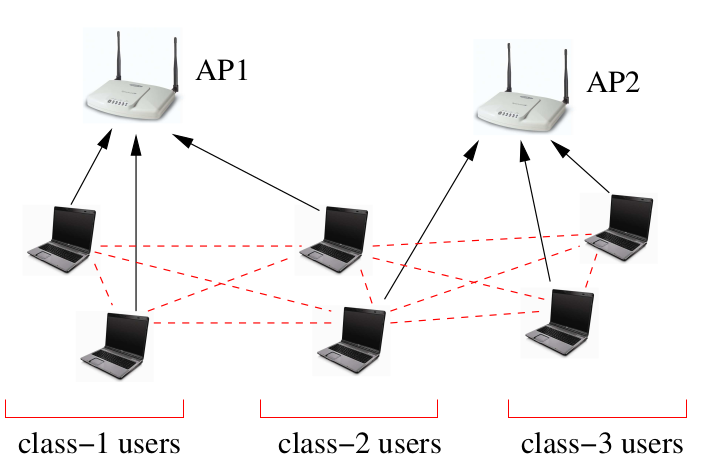
\includegraphics[width=\linewidth]{L26_Fig_1.png}
	\caption{A network with partial interference - A dashed line between two
users means that they sense each other.}
	\label{fig:1}
\end{figure} 

All 6 users are willing to transmit data packets to the access points 1 or 2; class-1 (resp. class-3) users interfere with users of classes 1 and 2 (resp. 2 and 3), whereas class-2 users interfere with all users. Two users of class 1 and 3 respectively can not sense each
other.

\section{System model}

We consider for example Local Area Networks (LANs) which are computer networks with relatively small geographic coverage (an office, a house, a part of a campus), and which constitutes the first crucial component of the Internet. \\

Transmissions in LANs are handled either on a cable (wired LANs) or on a radio channel (wireless LANs, also commonly called WiFi). Here we will focus on wireless LANs (analysis can be carried out similarly in the case of wired LANs). \\

In wireless LANs, users that are close to each other or that wish to transmit to the same receivers interfere in the sense that they cannot simultaneously transmit packets successfully. Two interfering users transmitting simultaneously are said to experience a collision. A collision is detected by a user at the end of the packet transmission when the corresponding receiver does not acknowledge a successful reception. \\

One of the most challenging problem in computer networking has been to design mechanisms so that interfering users could efficiently and fairly share the resource in a distributed manner.\\

\subsection{Random back-off algorithms} Currently the DCF is a version of the classical binary exponential back-off algorithm: after each successful transmission, a user picks a back-off counter uniformly in $\{0, . . . , t_{min}\}$, and after $m$ successive collisions uniformly in $\{0, . . . , 2^mt_{min}\}$.\\

In the following, we assume that the back-off distribution is always geometric (so as to keep a simple Markovian setting), although we could easily generalize the analysis to uniform distributions. With this assumption, each user transmits with a given probability $p$ at the beginning of each idle slot.
We consider the following generic way of adapting this probability: first the probability belongs to a countable set $\mathbb{B}$, after a successful transmission $p$ is updated to $S(p)$, and after a collision $p$ is updated to $C(p)$, where $S(·)$ (resp. $C(·)$) is a decreasing (resp. increasing) mapping from $\mathbb{B} \to \mathbb{B}$. Let $p_0 = \max\{p \in \mathbb{B}\}$.

\subsection{Interference model and user class} We consider a simple model for interference as follows: first, the N users
are classified according to their interference properties, i.e., two users belong to the same class if they interfere with (resp. are interfered with and by) the same set of users. Two users are of the same class if the corresponding links are located in the same geographic region (see for example the network of Figure 1). \\

Denote by $\mathbb{C}$ the set of user classes, and by $\mu_c$ the proportion of users of class $c$. $i \in c$ denotes the fact that user $i$ is of class $c$. Then interference between users of different classes is characterized by the inci-
dence matrix $A$ such that $A_{cd} = 1$ if class-c users interfere class-d users, and $A_{cd} = 0$ otherwise. 
Denote by $V_c = \{d \in C : A_{cd} = 1\}$ the set of classes of links interfering with class-$c$ links.
We say that the network has full interference if $A_{cd} = 1$ for all $c, d \in \mathbb{C}$ and has partial interference otherwise.

\subsection{Performance metrics}The performance metrics we aim at analyzing is the long-term throughput (the number of packets successfully transmitted per time unit) achieved by the users of various classes. We denote by $\gamma_c$ the throughput of class-$c$ users.\\

Deriving expressions for this performance metrics is notoriously difficult. This is due to the inherent interactions between users through interference.\\

In case of full interference, the network can be modeled as a simple system of particles with no randomly varying environment. However, to analyze a network with partial interference, the introduction of this varying environment is necessary.\\

\subsection{Model analysis}We consider a network of $N$ users and analyze the system at the beginning of each slot. Denote by $p_N
^i (k)/N$ the probability user $i$ becomes active at the end of the $k$-th slot, if idle (note the normalization of this probability by $1/N$ to be able to conduct the asymptotic analysis when $N$ grows large). For all $i, k, N , p_N^i (k) \in \mathbb{B}$.\\

To capture the network dynamics, we define a process $Z_N = \{Z_N (k), k \geq 0\}$ representing the state of classes during slot $k$. $Z_c^N (k) \in \{0, 1, 2\}$, where $Z_ c(k) = 0$ if and only if there is no transmitting user of class $c$, $Z_c^N (k) = 1$ if
and only if there is one successfully transmitting user of class c and $Z_c^N (k) = 2$ if and only if there is at least one user of class c currently in collision with another user in $V_c$ . Let $Z = \{0, 1, 2\}^{|C|}$ denote the state space of $Z$. We introduce the clear-to-send functions $C_c$ as follows : If $Z^N (k) = z$, a class-$c$ link is clear to send at the end of slot $k$ and $C_c (z) = 1$ if $z_d = 0$ for $d \in V_c$, otherwise $C_c (z) = 0$.\\

Modelling the network as $N$-particles system, the $i$-th user corresponds to the $i$-th particle with state describing the class of the user and the transmission probability at the end of the next idle slot $X_i^N (k) = (c_i , p^N_i (k)) \in \mathbb{X} = \mathbb{C} \times \mathbb{B}$.\\

The environment process: the evolution of the environment is determined by the states of all the particules through $v^N$ . The evolution of the $i$-th particle depends on whether or not the corresponding user senses the channel idle or not, i.e., $Z_i^N (k) = Z_c^N (k)$ for $i \in c$.

\subsection{Particle transitions} We first compute the transition probabilities for the various particles. The set $S$ of possible transitions is composed by two functions, the first one representing a successful transmission $p \to S(p)$ and the other one collisions $p \to C(p)$. Note that the class of a particle/user does not change.\\

Let $v_c^N (k) = \frac{1}{N}\sum_{i =1}^{N} \delta_{p_i^N(k)} \mathbb{1}_{c(i)=c}$ and $v^N (k) = (v_c^N (k))_{c\in\mathbb{C}}$.\\

Assume that at some slot $k$, the system is in state: \EQ{((c^N_i (k), p_i^N (k))_{i=1,...N}, v^N(k), Z^N(k))) = ((c_i, p_i )_{i=1,...,N} , \alpha, z)}

A class-$c$ user $i$ may have a transition at the end of slot $k$ only if $C_c (z) = 1$. In this case it can either initiate a successful transmission or experience a collision. If $C_c (z) = 1$, the event that none of the users in $c$ transmits at the end of slot $k$ is given by $D_c^N = \prod_{i \in c}{\mathbb{1}_{(NU_i > p_i)}} $, where the $U_i$ ’s are i.i.d. r.v. uniformly distributed on $[0, 1]$.\\

The event that user $i \in c$ accesses the channel with success at the end of slot $k$ is given by the indicator:
\EQ{\mathbb{1}_{\{NU_i \leq p_i\}}C_c(z)\prod_{j \in c,j \neq i}{\mathbb{1}_{\{NU_j > p_j\}}}\prod_{d \in V_c ,d \neq c}{(C_d(z)D_d^N + (1 - C_d (z)))}}

Averaging the above quantity gives the transition probability $F_S^N((c, p_i ), \alpha, z)/N$ corresponding to a successful transmission. For all $\alpha \in P(\mathbb{B})$ and all $f$ $B$-valued functions, define $\langle f, \alpha \rangle =  \sum_{p}f(p)\alpha(p)$. Moreover let $\alpha_c$ denote the restriction of $\alpha$ to users of class $c$. Let $I$ denote the identity function. Then:

\EQ{F_S^N ((c, p_i ), \alpha, z) =\frac{p_i}{1-\frac{p_i}{N}}C_c(z)\prod_{d in V_c}{(C_d(z)(e^{\langle Nlog(1− \frac{1}{N}),\alpha_d\rangle}- 1) + 1)}} 

Similarly, the event that user $i \in c$ experiences a collision at the end of slot $k$ is given by the indicator:
\EQ{\mathbb{1}_{\{NU_i \leq p_i\}}C_c(z)(1-\prod_{j \in c,j \neq i}{\mathbb{1}_{\{NU_j > p_j\}}\prod_{d \in V_c,d \neq c}{(C_d(z)D_d^N + (1-C_d(z)))}}}
and the transition probability $F_C^N((c, p_i ), \alpha, z)/N$ corresponding to a collision reads:
\EQ{F^N_C((c, p_i), \alpha, z) = p_iC_c(z)(1 -\frac{1}{1 - \frac{p_i}{N}}\prod_{d \in V_c, d \neq c}{(C_d(z)(e^{\langle Nlog(1-\frac{1}{N},\alpha_d\rangle} - 1) + 1)})}
We also need to introduce a virtual transition from $(c, p)$ to $(c, p)$ with transition rate $F^N_{\phi}((c, p_i), \alpha, z) = 1 - p_iC_c(z)$. 
With this virtual transition the sum of the transition rates sums to 1.\\

Since $Nlog(1-x/N)$ converges to $-x$, we obtain the following expressions for the asymptotic transition rates, $F_\phi((c, p_i), \alpha, z) = 1 - p_iC_c(z)$,
\EQ{F_S((c, p_i), \alpha, z) = p_iC_c(z)\prod_{d \in V_c}{(C_d(z)(e^{-\langle I,\alpha_d \rangle} - 1) + 1)}}
\EQ{F_C((c, p_i), \alpha, z) = p_iC_c(z)(1 -\prod_{d \in V_c}{(C_d(z)(e^{-\langle I,\alpha_d \rangle} - 1) + 1)}}

\subsection{Stationary throughputs}We are interested in deriving the stationary throughputs achieved by users of various classes. 
To do so, we derive the stationary distribution $Q_{st}$ and $\pi_{Q_{st}}$ of the particles and the background process.\\

To simplify the notation we write $Q_{st} = Q$ and $\pi_Q = \pi$. Also denote $Q^p_c = Q({c, p})$ the stationary proportion of users of class $c$ transmitting with probability $p$.\\

Consider the point process of returns to the set $A = \{z : C_c(z) = 1\}$. Let $T_1$ denote the first return time after time zero. 
%By the cycle formula (see
%(1.3.2) in [5]) we may express the steady state probability of a user in c successfully
%transmitting a packet by the mean time spent in the transmission
%state per cycle divided by the mean cycle length. The expectation is calculated
%with respect to the Palm measure of the point process of returns to A
%but in this Markovian case this just means starting on A with probability
%πA which is π renormalized to be a probability on A.
A user in $c$ can only go into a successful transmission state once per cycle;i.e. no other user in $c$ transmits and other users in $V_c$ are either blocked or remain silent. Hence the mean time per cycle spent in a transmission state is \EQ{\sum_{z \in A}{\pi^A(z)Lg(z)}} where \EQ{g(z) = p_c\prod_{d \in V_c,d \neq c}{(C_d(z)(e^{-p_d} - 1) + 1)}}
Moreover,\EQ{\sum_{z \in A}{\pi^A(z)E_z[T_1]} = \frac{1}{\pi(A)}} i.e. the intensity of the point process of visits to $A$. Finally the total throughput of the users of class $c$ is \EQ{\gamma_c =\sum_{z:C_c(z)=1}\pi(z)Lp_c\prod_{d \in V_c}{C_d(z)(e^{-p_d} - 1) + 1}} where
\EQ{p_c =\sum_{p \in \mathbb{B}}pQ^p_c}
which can be interpreted as the probability that a user of class c attempts
to use the channel at the end of an empty slot.

\end{document}
